\chapter{Apparence et disposition du texte}
\label{chap:apparence}


\section{Apparence du texte}

\subsection{Police de caractère}

\begin{itemize}
\item Par défaut, tous les documents {\LaTeX} utilisent la même police
  de caractère, {\fontfamily{cmr}\selectfont Computer Modern}
\item Aujourd'hui plus facile d'utiliser d'autres polices, surtout
  avec {\XeLaTeX}
  \begin{itemize}
  \item voir les fichiers d'exercices et les gabarits de
    \class{ulthese} pour des exemples
  \end{itemize}
\item Privilégier les polices de grande qualité et très complètes
  (lettres accentuées, grand choix de symboles)
  \begin{itemize}
  \item polices Postscript standards ou leurs clones du projet
    TeX~Gyre
  \end{itemize}
\item Peu de polices sont adaptées pour les mathématiques
  \begin{itemize}
  \item {\fontfamily{ppl}\selectfont Palatino},
    {\fontfamily{ptm}\selectfont Times}, \textrm{Lucida} (\$) sont des
    choix sûrs
  \end{itemize}
\item Voir le \autoref{tab:apparence:police} pour les commandes de
  changement d'attribut de la police de caractères.
\end{itemize}

\begin{table}
  \caption{Commandes de changement d'attribut de la police de
    caractères. Les commandes de la deuxième colonne s'appliquent à
    tout le texte qui suit. Celles de la troisième colonne
    s'appliquent uniquement au texte en argument.}
  \label{tab:apparence:police}
  \begin{tabularx}{\linewidth}{Xll}
    \toprule
    \textbf{famille} \\
    \textrm{romain} & \cmd{\rmfamily} & \cmdprint{\textrm{\meta{texte}}} \\
    \texttt{largeur fixe} & \cmd{\ttfamily} & \cmd{\texttt{\meta{texte}}} \\
    \textsf{sans empattements} & \cmd{\sffamily} & \cmdprint{\textsf{\meta{texte}}} \\
    \addlinespace[6pt]
    \textbf{forme} \\
    \textup{\rmfamily droit} & \cmd{\upshape} & \cmdprint{\textup{\meta{texte}}} \\
    \textit{\rmfamily italique} & \cmd{\itshape} & \cmdprint{\textit{\meta{texte}}} \\
    \textsl{penché} & \cmd{\slshape} & \cmdprint{\textsl{\meta{texte}}} \\
    \textsc{\rmfamily petites capitales} & \cmd{\scshape} & \cmdprint{\textsc{\meta{texte}}} \\

    \addlinespace[6pt]
    \textbf{série} \\
    \textmd{\rmfamily moyen} & \cmd{\mdseries} & \cmdprint{\textmd{\meta{texte}}} \\
    \textbf{\rmfamily gras} & \cmd{\bfseries} & \cmdprint{\textbf{\meta{texte}}} \\
    \bottomrule
  \end{tabularx}
\end{table}

\subsection{Taille de la police}

\begin{table}
  \caption{Commandes de changement de la taille de la police de caractère}
  \label{tab:apparence:taille}
  \begin{tabular}{ll}
    \toprule
    \cmd{\miniscule}$^\dagger$ & {\miniscule minuscule} \\
    \cmd{\tiny} & {\tiny très, très petit} \\
    \cmd{\scriptsize} & {\scriptsize très petit} \\
    \cmd{\footnotesize} & {\footnotesize plus petit} \\
    \cmd{\small} & {\small petit} \\
    \cmd{\normalsize} & {\normalsize normal} \\
    \cmd{\large} & {\large grand} \\
    \cmd{\Large} & {\Large plus grand} \\
    \cmd{\LARGE} & {\LARGE un peu plus grand} \\
    \cmd{\huge} & {\huge encore plus grand} \\
    \cmd{\Huge} & {\Huge énorme} \\
    \cmd{\HUGE}$^\dagger$ & {\HUGE vraiment énorme} \\
    \bottomrule
  \end{tabular}
  \hspace*{1em}{\footnotesize $^\dagger$ ajout de la classe
    \class{memoir} (et donc aussi de \class{ulthese})}
\end{table}

\subsection{Emphase}

\begin{itemize}
\item Une des propriétés les \emph{plus utilisées} dans le texte
\item Commande spécifique:
\begin{lstlisting}
\emph`\marg{texte}'
\end{lstlisting}
\item Par défaut: texte en italique dans texte droit et vice versa
  \begin{demo}
    \begin{texample}
\begin{lstlisting}
C'était un peu \emph{rough} par moments
\end{lstlisting}
      \producing
      C'était un peu \emph{rough} par moments
    \end{texample}
    \begin{texample}
\begin{lstlisting}
Il m'a dit: «\emph{C'était un peu \emph{rough}
par moments}»
\end{lstlisting}
      \producing
      Il m'a dit: «\emph{C'était un peu \emph{rough} par moments}»
    \end{texample}
  \end{demo}
\item Pas de commande pour souligner en {\LaTeX\dots} et ce n'est
  pas une omission!
\end{itemize}


\section{Portions de texte spéciales}

\subsection{Listes}

\begin{itemize}
\item Deux principales sortes de listes:
  \begin{enumerate}
  \item à puce avec environnement \Ie{itemize}
  \item numérotée avec environnement \Ie{enumerate}
  \end{enumerate}
\item Possible de les imbriquer les unes dans les autres
\item Marqueurs alors adaptés automatiquement
\end{itemize}

\begin{demo}
\begin{lstlisting}
\begin{itemize}
\item Deux principales sortes de listes:
  \begin{enumerate}
  \item à puce avec environnement \verb=itemize=
  \item numérotée avec environnement \verb=enumerate=
  \end{enumerate}
\item Possible de les imbriquer les unes
  dans les autres
\item Marqueurs adaptés automatiquement
\end{itemize}
\end{lstlisting}
\end{demo}

\begin{information}
  \begin{itemize}
  \item Mode français de \pkg{babel} redéfinit la puce de 1{\ier}
    niveau par défaut de {\textbullet} à {\textemdash}
  \item Pour changer, utiliser dans le préambule
\begin{lstlisting}
\frenchbsetup{
  ItemLabeli=\`\textit{commande}',
  ItemLabelii=\`\textit{commande}'}
\end{lstlisting}
  \item Voir les ressources pour une vaste sélection de symboles
  \end{itemize}
\end{information}

\begin{conseil}
  \begin{itemize}
  \item {\LaTeX} permet de configurer à peu près toutes les facettes
    de la présentation des listes (puces, alignement, espacement).
  \item Plusieurs paquetages facilitent la configuration.
  \item Nous suggérons \pkg{enumitem} pour une configuration simple.
  \end{itemize}
\end{conseil}

\subsection{Texte centré}

\begin{center}
  Pour obtenir du texte centré on utilise l'environnement
  \Ie{center}
\end{center}

\begin{lstlisting}
\begin{center}
  Pour obtenir du texte centré on utilise
  l'environnement \verb=center=
\end{center}
\end{lstlisting}

{\centering ou encore la commande \cmd{\centering}}

\begin{lstlisting}
\centering ou encore la commande \verb=\centering=
\end{lstlisting}

\subsection{Citations}

Deux environnements de citation dans {\LaTeX} (et \class{ulthese})
\begin{enumerate}
\item \Ie{quote} pour les citations courtes, quelques lignes seulement
  \begin{itemize}
  \item retrait à gauche et à droite
  \end{itemize}
\item \Ie{quotation} pour les citations plus longues se comptant
  en paragraphes
  \begin{itemize}
  \item retrait à gauche et à droite
  \item gestion des marques de paragraphes
  \end{itemize}
\end{enumerate}

\subsection{Notes de bas de page}

\begin{itemize}
\item Note de bas de page insérée avec la commande
\begin{lstlisting}
\footnote`\marg{texte de la note}'
\end{lstlisting}
\item Commande doit suivre immédiatement le texte à annoter
\item Méthode recommandée
\begin{lstlisting}[emph=footnote]
... fera remarquer que Pierre Lasou\footnote{%
  Spécialiste en ressources documentaires} %
fut d'une grande aide dans la préparation de ...
\end{lstlisting}
\item Numérotation et disposition automatiques
\end{itemize}

\subsection{Code source}

\begin{itemize}
\item Environnement \Ie{verbatim}
\begin{lstlisting}
\begin{verbatim}
Texte disposé exactement tel qu'il est tapé
dans une police à largeur fixe
\end{verbatim}
\end{lstlisting}
\item Commande \cmd{\verb} dont la syntaxe est
\begin{lstlisting}
\verb`\meta{c}' `\meta{source}' `\meta{c}'
\end{lstlisting}
  où \meta{c} est un caractère quelconque ne se trouvant pas dans
  \meta{source}
\item Pour usage plus intensif, voir le paquetage \pkg{listings}.
\item Plus de détails à la \autoref{sec:trucs:listings}.
\end{itemize}


\section{B.a.-ba des mathématiques}

\subsection{Préliminaires}

\begin{itemize}
\item Décrire des équations mathématiques requiert un «langage»
  spécial
  \begin{itemize}
  \item il faut informer {\LaTeX} que l'on passe à ce langage
  \item par le biais de modes mathématiques
  \end{itemize}
\item Important d'utiliser un mode mathématique
  \begin{itemize}
  \item règles de typographie spéciales (constantes vs variables,
    disposition des équations, numérotation, etc.)
  \item espaces entre les symboles et autour des opérateurs gérées
    automatiquement
  \end{itemize}
\item Vous voulez utiliser le paquetage \pkg{amsmath}
\begin{lstlisting}
\usepackage{amsmath}
\end{lstlisting}
  \begin{itemize}
  \item lire la documentation de ce paquetage pour connaître toutes
    ses fonctionnalités
  \end{itemize}
\end{itemize}

\subsection{Modes mathématiques}

\begin{enumerate}
\item «En ligne» directement dans le texte comme
  $(a + b)^2 = a^2 + 2ab + b^2$ en plaçant l'équation entre \verb=$ $=
\begin{lstlisting}
«En ligne» directement dans le texte
comme $(a + b)^2 = a^2 + 2ab + b^2$
\end{lstlisting}
\item «Hors paragraphe» séparé du texte principal comme
  \begin{displaymath}
    \int_0^\infty f(x)\, dx = \sum_{i = 1}^n \alpha_i e^{x_i} f(x_i)
  \end{displaymath}
  en utilisant divers types d'environnements
\begin{lstlisting}
«Hors paragraphe» séparé du texte principal comme
\begin{displaymath}
  \int_0^\infty f(x)\, dx =
  \sum_{i = 1}^n \alpha_i e^{x_i} f(x_i)
\end{displaymath}
\end{lstlisting}
\end{enumerate}

\begin{conseil}
  Les équations, en ligne ou hors paragraphe, font partie intégrante
  de la phrase. Les règles de ponctuation usuelles s'appliquent donc
  aux équations.

  \fbox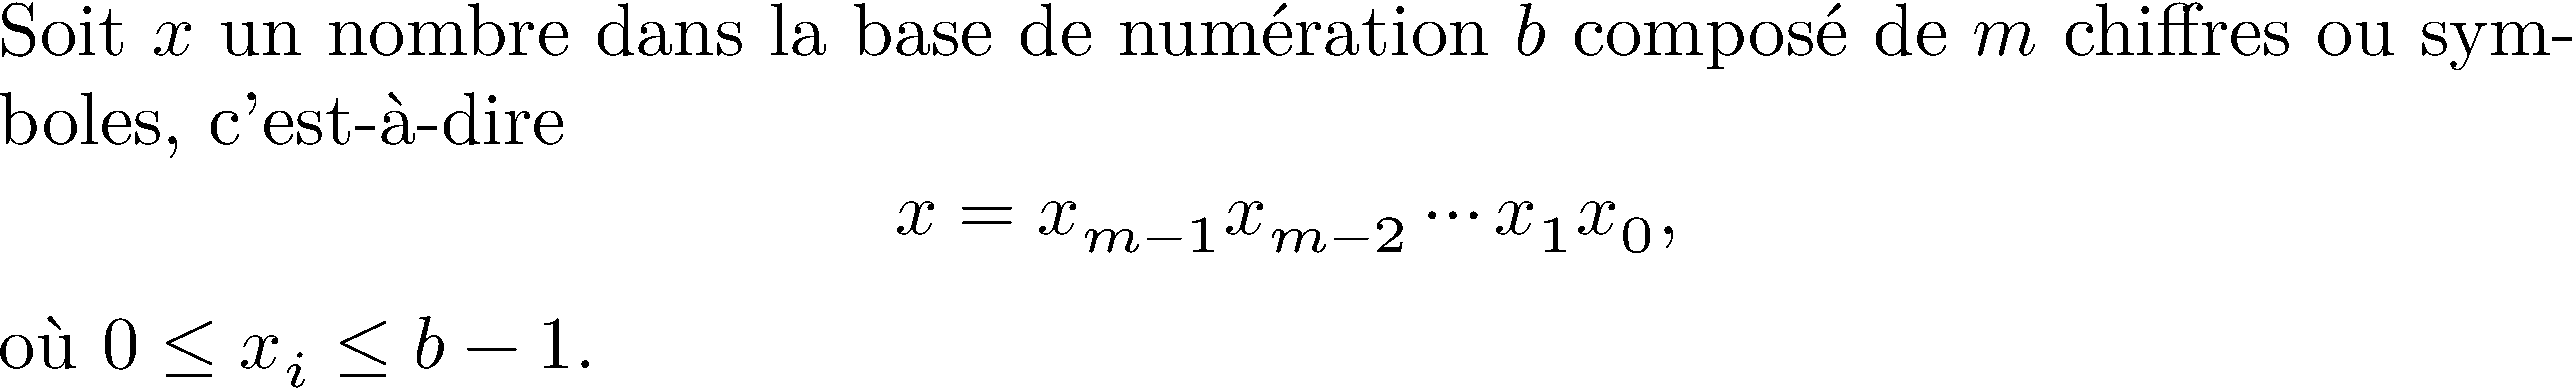
\includegraphics[width=0.95\linewidth]{ponctuation}
\end{conseil}

\subsection{Quelques règles de base du mode mathématique}

\begin{itemize}
\item En mode mathématique, {\TeX} respecte automatiquement la
  convention d'écrire les constantes en \rmfamily{romain} et les
  variables en \textit{italique}
  \begin{demo}
    \begin{texample}
\begin{lstlisting}
$z = 2a + 3y$
\end{lstlisting}
      \producing
      $z = 2a + 3y$
    \end{texample}
  \end{demo}
\item Espace entre les éléments géré automatiquement, peu importe le
  code source
  \begin{demo}
    \begin{texample}
\begin{lstlisting}
$z=2 a+3 y$
\end{lstlisting}
      \producing
      $z=2 a+3 y$
    \end{texample}
  \end{demo}
\item \epmh{Ne pas} utiliser le mode mathématique pour obtenir du
  texte en italique!
  \begin{demo}
    \begin{texample}
\begin{lstlisting}
\emph{xyz}
\end{lstlisting}
      \producing
      \rmfamily\emph{xyz}
    \end{texample}
    \begin{texample}
\begin{lstlisting}
$xyz$
\end{lstlisting}
      \producing
      $xyz$
    \end{texample}
  \end{demo}
\item Utiliser la commande \cmd{\text} de \pkg{amsmath} pour
  obtenir du texte à l'intérieur du mode mathématique
  \begin{demo}
    \begin{texample}
\begin{lstlisting}
$x = 0 \text{ si } y < 2$
\end{lstlisting}
      \producing
      $x = 0 \text{ si } y < 2$
    \end{texample}
  \end{demo}
\item Le \autoref{chap:mathematiques} fournit plus de détails.
\end{itemize}

\subsection{Environnements pour les équations hors paragraphe}

\begin{itemize}
\item Équation d'une seule ligne numérotée: \Ie{equation}.
  \renewcommand{\theequation}{\arabic{equation}}
  \begin{eqxample}
\begin{lstlisting}
\begin{equation*}
  a = b
\end{equation*}
\end{lstlisting}
    \producing
    \begin{equation*}
      a = b
    \end{equation*}
  \end{eqxample}

  \begin{eqxample}
\begin{lstlisting}
\begin{equation}
  a = b
\end{equation}
\end{lstlisting}
    \producing
    \begin{equation}
      a = b
    \end{equation}
  \end{eqxample}

\item Équation d'une seule ligne non numérotée: \Ie{displaymath}, \Ie{equation*}.
\item Série d'équations alignées, généralement sur \verb|=|
\end{itemize}


%%%
%%% Exercices
%%%

\section{Exercice}
\label{sec:apparence:exercices}

\begin{exercice}
  \begin{enumerate}
  \item Ouvrir le fichier \fichier{exercice\_complet.tex} et en
    étudier le code source, puis le compiler.
  \item Supprimer l'option \code{article} au chargement de la classe
    et compilier de nouveau le document. Observer l'effet de cette
    option.
  \item Effectuer les modifications suivantes au document.
    \begin{enumerate}[a)]
    \item Dernier paragraphe de la première section, placer toute la
      phrase débutant par \code{«De simple dérivé»} à l'intérieur
      d'une commande \cmd{\emph}.
    \item Changer la puce des listes pour le caractère \code{\$>\$}.
    \end{enumerate}
  \end{enumerate}
\end{exercice}

%%% Local Variables:
%%% mode: latex
%%% TeX-engine: xetex
%%% TeX-master: "formation_latex_UL-partie_2"
%%% coding: utf-8
%%% End:
